\documentclass[12pt,a4paper]{article}
\usepackage[utf8]{inputenc}
\usepackage[english]{babel}
\usepackage{amsmath}
\usepackage{amsfonts}
\usepackage{amssymb}
\usepackage{graphicx}
\usepackage{subcaption}

\author{Sven Eriksson}
\title{Writeup for Behavioral Cloning project \\ \large{Part of Udacity self driving car nanodegree}}

\setlength{\parindent}{0pt} % Default is 15pt.
\usepackage{parskip}


\begin{document}
\maketitle

\section*{The goals / steps of this project are the following}
\begin{itemize}
\item Use the simulator to collect data of good driving behavior
\item Build, a convolution neural network in Keras that predicts steering angles from images
\item Train and validate the model with a training and validation set
\item Test that the model successfully drives around track one without leaving the road
\item Summarize the results with a written report
\end{itemize}

I have done all of these things and the purpose of this report is to describe that.

\section{Files Submitted \& Code Quality}

The code I wrote for this project is located in the folder 'code'. The file 'drive.py' for driving the car in autonomous mode is located directly in the top folder. In the same top folder one can also find this report, 'writeup\_report.pdf' and 'model.h5' that contains the trained neural network.

My code is devided up into 3 files. 'model.py' that describe the model and calls the training functions from Keras. 'dataLoader.py' that reads the comma separated files containing the names and angles for all images. 'dataLoader.py' does also divede the dataset into a training and validation set. Finally it also contains the code for creating the generators for training and validation. The last file is 'config.py' that contains the parameters I changed during training the network.

All three files contains comments and are structured in a way to make it easy to understand.

\section{Model Architecture and Training Strategy}
My model is based on the one NVidia used in their article 'End to End Learning for Self-Driving Cars' \cite{DBLP:journals/corr/BojarskiTDFFGJM16}.

I did a few modifications to it in order to adapt it to this task and to try out a few things for testing and learning purposes.

\subsection{Network architecture}

\subsubsection{Normalization and grayscale}
All elements in the three color layers, red, blue, and green, were normalized to be around zero by dividing them by 255 and subtracting 0.5 from the result.

A forth layer containing the image in grayscale was created by taking the average of the three color layers in each pixel. I am aware that the network can learn to see the images in grayscale by in each pixel having the same value for each color layer. But I wanted to test how to concatenate layers and to see if it helped by manually defining this grayscale layer. I don't think it did as the result was similar and the training time was slightly longer.

Theese four layers were then used together as input for the convulisional part of the neural network.

\subsubsection{Convultional layers}
Input size is 66 pixels as hegith by 320 pixels as width by 4 'colors'. The activation function for these layers is 'relu'. This input is wider than the one NVidia used and has an additional 'color'. So I decided to increase the feature depth in each layer. This has probably increased the training time but it also allows for potentially more features.

\begin{tabular}{| l | l | l |}
\hline
Feature depth & Filer & Stride \\
\hline
36 & 5 by 5 & 2 in both directions \\
48 & 5 by 5 & 2 in both directions \\
64 & 5 by 5 & 2 in both directions \\
80 & 5 by 5 & 1 in both directions \\
80 & 5 by 5 & 1 in both directions \\
\hline
\end{tabular}

Output size is 1 pixels as hegith by 33 pixels as width by 80 as feature depth. This is then flattened and used as input to the following fully connected layers.

\subsubsection{Fully connected layers}
For the fully connected layers I experimented with a few different activation functions and even though I didn't really see any difference I ended up using 'tanh' for all fully connected layers except the output layer that had no activation function.

There fully connected layers are 50\% larger than those in the NVidia article \cite{DBLP:journals/corr/BojarskiTDFFGJM16}. This is done to deal with the input to the fully connected layers that is nearly twice the size of the one found in NVidia's article.

\begin{tabular}{| l | l |}
\hline
Number of neurons & Type\\
\hline
150 & Internal layer\\
75 & Internal layer \\
15 & Internal layer \\
1 & Output layer \\
\hline
\end{tabular}


\subsection{Attempts to reduce overfitting in the model}
An attempt to reduce overfitting has been done by adding a dropout layer between allmost all layers.

The model was trained and validated on different but similar data sets as I randomly took images from the same track.

\subsection{Model parameter tuning}
The model used an adam optimizer, so the learning rate was not tuned manually. 

The only value that was tuned was the adjustment angle for images from the right and left camera. But that is modifing a parameter for the training data rather than the model.

\subsection{Appropriate training data}
Training data was randomly picked from my several runs with manual control on the easier of the two tracks. 

\section{Model Architecture and Training Strategy}

\subsection{Solution Design Approach}

As I had previously encountered the NVidia article in my work I used the network described there as a starting point. 

I added dropout layers to prevent overfitting. All layers were also increased in order to adjust for the difference in input size between NVidia's article and our simulation.

At the end of the process, the vehicle is able to drive autonomously around the track without leaving the road.

\subsection{Creation of the Training Set \& Training Process}

I focused on driving somewhat in the center of the road during all runs and used a adjustment angle images from the right and left camera. There adjustment angles were tuned in such a way so that the network would learn to steer towards the middle should it ever see a similar image.

For a visualization of the raw images given to the network see figure \ref{fig:images}. The network does then crop the images in a way that can be seen in figure \ref{fig:images_crop}.

For each image I created a flipped copy by the time of loading it. The flipped and unflipped images were independntly picked for training and validation and for different batches. When creating a flipped copy of an image I also created a flipped copy of the recorded angle, with our without adjustment angle depending on the which camera that took the image. The distribution of angles of this augmented dataset can be seen in figure \ref{histogram}.


\begin{figure}
    \centering
    \begin{subfigure}[b]{0.3\textwidth}
        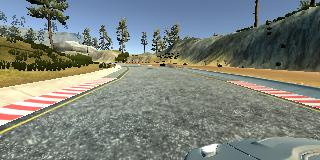
\includegraphics[width=\textwidth]{left.jpg}
        \caption{Image from the left 'camera'.}
        \label{fig:left}
    \end{subfigure}
    ~ %add desired spacing between images, e. g. ~, \quad, \qquad, \hfill etc. 
      %(or a blank line to force the subfigure onto a new line)
    \begin{subfigure}[b]{0.3\textwidth}
        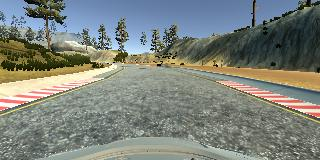
\includegraphics[width=\textwidth]{center.jpg}
        \caption{Image from the center 'camera'.}
        \label{fig:center}
    \end{subfigure}
    ~ %add desired spacing between images, e. g. ~, \quad, \qquad, \hfill etc. 
    %(or a blank line to force the subfigure onto a new line)
    \begin{subfigure}[b]{0.3\textwidth}
        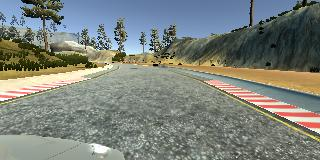
\includegraphics[width=\textwidth]{right.jpg}
        \caption{Image from the right 'camera'.}
        \label{fig:right}
    \end{subfigure}
    \caption{Raw images from the 3 'cameras'. All are 160 by 320 pixels.}\label{fig:images}
\end{figure}

\begin{figure}
    \centering
    \begin{subfigure}[b]{0.3\textwidth}
        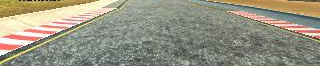
\includegraphics[width=\textwidth]{left_crop.jpg}
        \caption{Image from the left 'camera'.}
        \label{fig:left_crop}
    \end{subfigure}
    ~ %add desired spacing between images, e. g. ~, \quad, \qquad, \hfill etc. 
      %(or a blank line to force the subfigure onto a new line)
    \begin{subfigure}[b]{0.3\textwidth}
        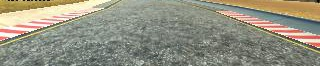
\includegraphics[width=\textwidth]{center_crop.jpg}
        \caption{Image from the center 'camera'.}
        \label{fig:center_crop}
    \end{subfigure}
    ~ %add desired spacing between images, e. g. ~, \quad, \qquad, \hfill etc. 
    %(or a blank line to force the subfigure onto a new line)
    \begin{subfigure}[b]{0.3\textwidth}
        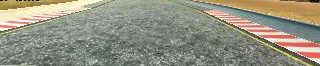
\includegraphics[width=\textwidth]{right_crop.jpg}
        \caption{Image from the right 'camera'.}
        \label{fig:right_crop}
    \end{subfigure}
    \caption{Cropped images from the 3 'cameras'. All are 66 by 320 pixels.}\label{fig:images_crop}
\end{figure}

\begin{figure}
	\centering
	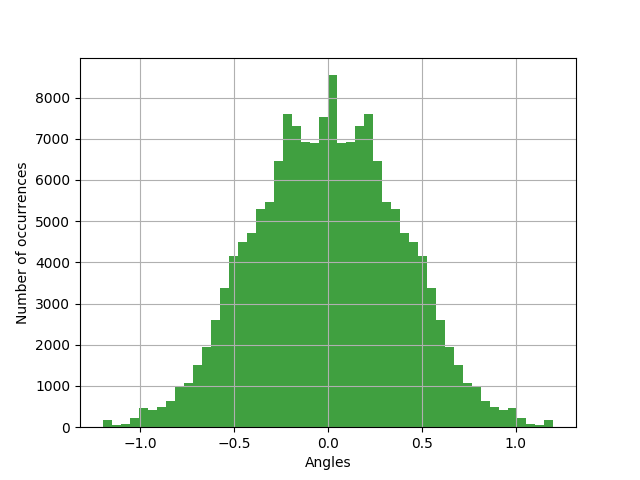
\includegraphics[scale=1]{histogram.png}
	\caption{Histogram of the distrubition of angles in my augmented dataset. It is symmetrical due to how it was created with flipped images.}
\label{histogram}
\end{figure}

When the model failed to drive as intended I gathered more of the same kind of data and also tuned to adjustment angle to teach the network to stay towards the middle.

The successful runs around the easy track can be seen in the video clips in this github repository.

\bibliography{bibtex}{}
\bibliographystyle{plain}

\end{document}